% !TeX program = xelatex
\documentclass[paper=a4,oneside,abstract,parskip=half]{scrartcl}

\usepackage[T1]{fontenc}
\usepackage[ngerman]{babel}
\usepackage{graphicx}
\usepackage{csquotes}
\usepackage{booktabs}
\usepackage{siunitx}
\sisetup{separate-uncertainty = true,locale=DE}
\usepackage{float}
\usepackage{placeins}
\usepackage{xcolor}
\definecolor{mygreen}{RGB}{34,139,34}
\usepackage{amsmath}
\usepackage{circuitikz}
\usepackage[backend=biber,
date=long,
style=iso-numeric,
autolang=other,
%bibencoding=UTF8
]{biblatex}

\DeclareFieldFormat{labelnumberwidth}{[#1]}
\setcounter{biburllcpenalty}{7000}
\setcounter{biburlucpenalty}{8000}

\usepackage[hidelinks]{hyperref}

% Figure lookup order:
% 1) local documentation assets
% 2) analysis exports
% 3) raw/shared data figures
\graphicspath{{figures/}{../Analysis/exports/figures/}{../Data/figures/}{../Data/raw}{../Data/tables}{../Data/literature}}

\addbibresource{bib/myLibrary.bib}

\title{Verzögerungszeit eines 74HC00 NAND Gatters}
\subject{Messbericht}
\titlehead{}
\author{Your name and everybody else}
\date{Messung: 9. und 16. April 2026 / Bericht: 20. April 2026}

\begin{document}
\shorthandoff{"}
\maketitle
\begin{abstract}
\noindent 

\noindent For template purposes, different kinds of text, tables and figures are present here. Feel free to change anything. First of all, change the language to your liking.

\end{abstract}

\section{Introduction}

This report documents the experimental setup, measurements, and analysis results.

All source data are kept in the repository under \texttt{../Data/}, and plots/tables generated in notebooks are exported to \texttt{../Analysis/exports/} for direct inclusion in this document.


\section{Method and Workflow}

\subsection{Data Organization}
Raw inputs are stored in \texttt{../Data/raw/}. Cleaned or transformed inputs are stored in \texttt{../Data/processed/}.

\subsection{Analysis Workflow}
Jupyter notebooks in \texttt{../Analysis/} perform calculations and export figures/tables to \texttt{../Analysis/exports/}.

\subsection{Documentation Workflow}
This LaTeX project references local and exported assets via \texttt{\textbackslash graphicspath}.


\section{Examples}

Here, you can find several example of typical elements I use in my reports.
\subsection{Circuit Example}

\begin{figure} [!htb]
\begin{center}
\begin{circuitikz}
  \draw
  (0,0) to[battery1, l=$V_s$] (0,3)
        to[R, l=$R_1$] (3,3)
        to[C, l=$C_1$] (3,0)
        -- (0,0);
\end{circuitikz}
\end{center}
\caption{Some kind of circuit.}
\label{fig:circuit}
\end{figure}

This line is referencing the circuit in figure \ref{fig:circuit} right above.
\subsection{Figure Example}

\begin{figure}[!htb] %alternatively [H] for forcing "here"
\begin{center}
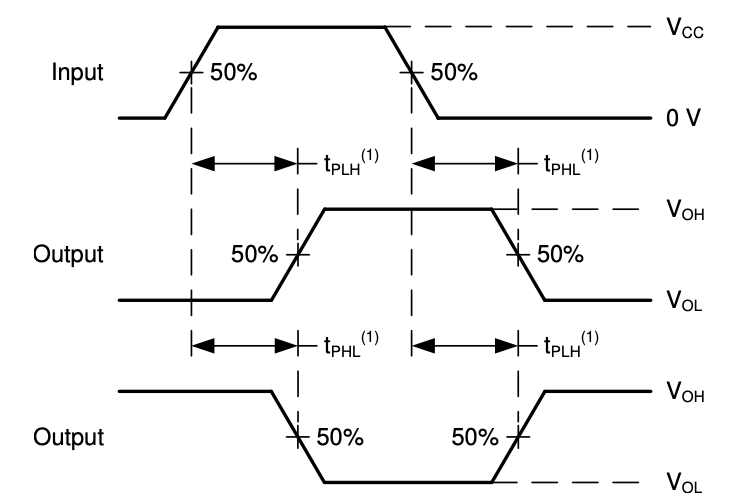
\includegraphics[width=0.5\textwidth]{
Verzoegerungszeit.png
}
\end{center}
\caption{Definition der Verzögerungszeiten aus dem Datenblatt des IC \protect\cite[Figure 7-2]{SNx4HC00}}
\label{fig:messprinzip}
\end{figure}
In Abbildung \ref{fig:messprinzip} aus dem Datenblatt ist dargestellt wie die Verzögerungszeiten $t_{\textrm{pLH}}$ und $t_{\textrm{pHL}}$ definiert sind \cite[Figure 7-2]{SNx4HC00}.

\subsection{Table Example}
This is how you can include a table:

\begin{table}[!htb] %alternatively [H] for forcing "here"
\centering
\begin{tabular}{c c c c}
\hline
{$t_{\mathrm{pLH}}$ bei \qty{2}{\volt}} &
{$t_{\mathrm{pHL}}$ bei \qty{2}{\volt}} &
{$t_r$ bei \qty{2}{\volt}} &
{$t_f$ bei \qty{2}{\volt}} \\
\hline
\qty{258,6}{\ns} & \qty{257,8}{\ns} & \qty{17,2}{\ns} & \qty{19,1}{\ns} \\
\hline
\end{tabular}
\caption{Messwerte der Verzögerungszeit bei \qty{2}{\volt}}
\label{tab:messwerte2v}
\end{table}

This line is just to show quoting table \ref{tab:messwerte2v}.

\printbibliography
\end{document}